\documentclass{article}

% AlpaSim technical report (nuPlan track), team amanupg. Built on the organisers' template
% (neurips_2026.sty and README.md in this folder, copied from the organisers' package); not a NeurIPS submission.
% DRAFT 2026-10-21. Items marked TODO need Aman's input or the official result of the q:3 entry (tag v6).
\PassOptionsToPackage{numbers}{natbib}
\usepackage[preprint]{neurips_2026}
\makeatletter
\renewcommand{\@noticestring}{}
\makeatother

\usepackage[utf8]{inputenc}
\usepackage[T1]{fontenc}
\usepackage{hyperref}
\usepackage{booktabs}
\usepackage{graphicx}
\usepackage{xcolor}
\usepackage{amsmath}
\usepackage{tikz}
\usetikzlibrary{positioning,arrows.meta,fit}

\newcommand{\todo}[1]{\textcolor{red}{[TODO: #1]}}

\title{A Learned Critic in the Loop: Plan Substitution and Stall Rescue for a Fine-Tuned Latent TransFuser\\
\large AlpaSim E2E Closed Loop Challenge Technical Report (nuPlan track)}

\author{
  Team amanupg \\
  \todo{author name(s), organization} \\
  \texttt{\todo{contact email}}
}

\begin{document}
\maketitle

\begin{abstract}
Our nuPlan-track entry combines a planner and a critic, both built from public resources. The planner is the
public py123d\_garage latent TransFuser, fine-tuned for 15 epochs on public nuPlan logs. The critic is the public
GTRS-Dense trajectory scorer, which rates the planner's plan against a 16{,}384-trajectory vocabulary. It replaces
the plan only when a nearby alternative scores clearly higher (\emph{plan substitution}). It also replaces it when
the plan barely moves and a clearly safe, better-scoring moving path exists (\emph{stall rescue}). A closed-loop
failure analysis motivated stall rescue: after substitution, low-progress scenes cost more score than all crashes
combined. On 754 local nuPlan scenes, compared per scene and including 193 scenes never used for any choice, the
full system raises the mean scene score from 0.724 (public checkpoint) to 0.852 (+0.128, 90\% bootstrap interval
[+0.108,\,+0.149]). Off-road failures fall from 105 to 36, and at-fault collisions stay level. \todo{official
result of v6: scene score, PCS, at-fault distance.} We also report what did not help: more fine-tuning data, longer
fine-tuning, weight averaging, and wider rescue thresholds.
\end{abstract}

\section{Method summary}
The policy has three stages (Fig.~\ref{fig:system}). (1) A fine-tuned py123d\_garage latent TransFuser
(LTF)~\cite{py123d} plans 4\,s ahead from the front cameras, ego status and the route. (2) A GTRS-Dense
scorer~\cite{simscale,gtrs} predicts, for the plan and for every vocabulary trajectory, the probability of no
at-fault collision (NC), drivable-area compliance (DAC) and ego progress (EP). It then decides whether to keep the plan,
substitute a nearby trajectory, or rescue a stalled plan. (3) Plans the critic kept, and which are near-straight, are
time-scaled by 1.10, the organisers' trajectory time warp. Every stage is inference-only at test time. The only
training is the planner's fine-tune.

\begin{figure}[h]
\centering
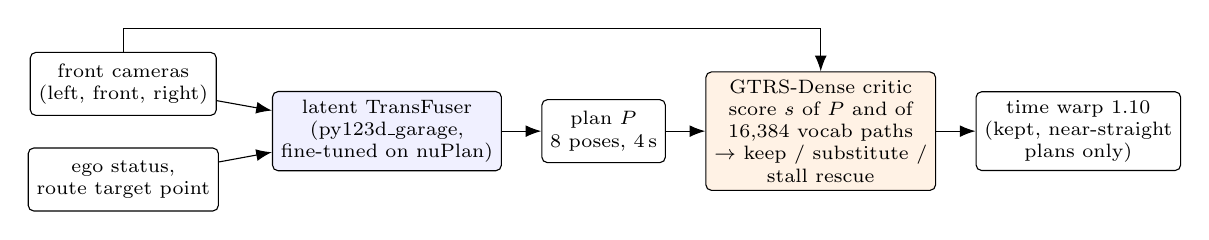
\begin{tikzpicture}[node distance=4mm and 5mm, font=\scriptsize,
  box/.style={draw, rounded corners=2pt, align=center, minimum height=8mm, inner sep=3pt},
  ar/.style={-{Latex[length=2mm]}}]
\node[box] (cam) {front cameras\\(left, front, right)};
\node[box, below=of cam] (ego) {ego status,\\route target point};
\node[box, right=7mm of cam, yshift=-6mm, fill=blue!6] (ltf) {latent TransFuser\\(py123d\_garage,\\fine-tuned on nuPlan)};
\node[box, right=of ltf] (plan) {plan $P$\\8 poses, 4\,s};
\node[box, right=of plan, fill=orange!10] (judge) {GTRS-Dense critic\\score $s$ of $P$ and of\\16{,}384 vocab paths\\$\rightarrow$ keep / substitute /\\stall rescue};
\node[box, right=of judge] (tw) {time warp 1.10\\(kept, near-straight\\plans only)};
\draw[ar] (cam) -- (ltf); \draw[ar] (ego) -- (ltf); \draw[ar] (ltf) -- (plan); \draw[ar] (plan) -- (judge);
\draw[ar] (judge) -- (tw);
\draw[ar] (cam.north) -- ++(0,3mm) -| (judge.north);
\end{tikzpicture}
\caption{System. The critic (orange) sees the same camera frames as the planner. Only the fine-tune, the
substitution and rescue rules, and their thresholds are ours; all networks are public.}
\label{fig:system}
\end{figure}

\section{Policy description}
\textbf{Planner.} The py123d\_garage latent TransFuser (ResNet-34 image encoder, latent BEV query in place of
LiDAR) takes the front cameras, ego velocity and acceleration, a driving command, and a target point 45\,m
along the route. It outputs 8 poses at 0.5\,s. We start from the public checkpoint \texttt{resnet34\_v0.1.0/model\_0014}
and fine-tune it as described in Sec.~\ref{sec:resources}.

\textbf{Critic score.} For a trajectory $\tau$, GTRS-Dense outputs logits for NC, DAC and EP. Following the
organisers' GTRS sample, we score $s(\tau)=\log\sigma(\mathrm{NC})+\log\sigma(\mathrm{DAC})+3\log\sigma(\mathrm{EP})$,
i.e. the log of $\mathrm{NC}\cdot\mathrm{DAC}\cdot\mathrm{EP}^3$. The planner's plan is converted to the vocabulary's
format and scored in the same forward pass as the 16{,}384 vocabulary trajectories. One critic call per planning step
covers all of them.

\textbf{Plan substitution.} Let $g$ be the best-scoring vocabulary trajectory whose every pose lies within $r=3$\,m of
the plan's corresponding pose. The plan is replaced by $g$ only if $s(g)-s(P)>m=3$, a factor of $e^3\approx20$ in
$\mathrm{NC}\cdot\mathrm{DAC}\cdot\mathrm{EP}^3$. The radius keeps the critic to local corrections of the planner's intent
(it cannot pick a different manoeuvre), and the margin makes it override only when it is confident. Without the
radius, in our first closed-loop tests, the critic (trained on NAVSIM) picked paths that did worse than the planner's.

\textbf{Stall rescue.} After substitution, scenes where the car barely moved while the recorded driver pulled away
cost more score than all collision, off-road and corridor failures together. If the chosen trajectory ends within
3\,m of the car after 4\,s, we consider the best-scoring vocabulary trajectory anywhere that moves at least 3\,m and
whose NC and DAC probabilities both exceed 0.9. It replaces the plan if its score is higher by more than 1. The
probability floor keeps the rescue from trading a stop for a risky move. About 5\% of planning steps are stalls, and
a third of those are rescued.

\textbf{Time warp.} Plans the critic kept, with heading change below $10^\circ$ over 4\,s, are time-scaled by 1.10, the
organisers' rule from their GTRS sample. Plans the critic substituted are not scaled: scaling its picks tripled at-fault collisions locally.

\section{Resources and training}
\label{sec:resources}
\textbf{All resources are public.}
\textbf{Pretrained weights:} the py123d\_garage checkpoint \texttt{resnet34\_v0.1.0/model\_0014} and sensor rig
(Hugging Face \texttt{kesai-labs/py123d\_garage\_pretrained\_checkpoints}, Apache-2.0)~\cite{py123d}, and the GTRS-Dense
checkpoint \texttt{gtrs\_dense\_resnet\_sim\_reward\_navhard} (Hugging Face \texttt{OpenDriveLab/SimScale},
Apache-2.0)~\cite{simscale}.
\textbf{Code:} py123d\_garage v0.1.1 (Apache-2.0), the organisers' GTRS-Dense inference wrapper and trajectory vocabulary
\texttt{navsim\_16384.npy} (NVlabs/alpasim \texttt{e2e\_challenge}, Apache-2.0), and \texttt{alpasim\_grpc} (Apache-2.0).
\textbf{Data:} nuPlan train and val logs in py123d's 123D format (Hugging Face \texttt{kesai-labs/nuplan}, under the
nuPlan terms of use)~\cite{nuplan}. No test-split data was used. \todo{confirm the exact nuPlan dataset licence name for
the report.} Local closed-loop evaluation used the public nuPlan-track navtest assets
(\texttt{OpenDriveLab/AlpasimChallenge2026\_nuplan\_track}) only for evaluation, never for training.

\textbf{Fine-tune.} We used py123d\_garage's own nuPlan post-training recipe (\texttt{ltf\_nuplan\_trainval}),
initialised from the public checkpoint. The data was 430 logs spread evenly over the train and val index (362 train,
68 val; 108{,}414 samples), with three front cameras and no LiDAR. Training ran for 15 epochs (the end of a cosine
warm-restart cycle) with batch 64 on one workstation GPU: about 1\,h of training after 5\,h of data download and
caching, all on node-local disk.

\section{Runtime and reproducibility}
\textbf{Inference.} The planner and the critic run on the same GPU in one process. With two concurrent sessions,
the driver process peaked at 8.3\,GiB (\texttt{nvidia-smi}), half the 16\,GiB limit. The critic adds one ResNet
forward pass and one scoring pass over 16{,}385 trajectories per planning step. \todo{per-call latency on H100.}
The submission image is 12.8\,GB, offline, with all weights baked in.

\textbf{Local evaluation protocol.} The simulator is deterministic: reruns of a configuration on the same GPU type give
identical scene scores. Noise therefore comes from scene sampling, not reruns, so we compared configurations per scene
on a growing pool, using 90\% bootstrap intervals. Scenes came from public navtest parts in three groups. \emph{Tuning}
(300 scenes) was used to choose thresholds. \emph{Held-out} (261) was used only to confirm. \emph{Fresh} (193, two
further parts) was never looked at before a change was frozen. A change was adopted only if positive on all three.
The final image was re-run in closed loop and reproduced the tested configuration on 200 of 200 scenes.

\begin{table}[h]
\centering\small
\begin{tabular}{lcc}
\toprule
Configuration (754 local scenes) & mean scene score & step gain [90\%] \\
\midrule
public py123d checkpoint (\texttt{model\_0014}) & 0.724 & -- \\
+ critic substitution ($m=3$, $r=3$\,m) + time warp & 0.798 & +0.075 [+0.058, +0.092] \\
+ fine-tuned planner & 0.809 & +0.011 [$-$0.002, +0.025] \\
+ stall rescue at 1\,m & 0.839 & +0.030 [+0.020, +0.039] \\
\textbf{+ stall rescue at 3\,m (final)} & \textbf{0.852} & \textbf{+0.013 [+0.008, +0.019]} \\
\bottomrule
\end{tabular}
\caption{Local closed-loop results, each step paired against the previous row on the same 754 scenes. Final vs public:
+0.128 [+0.108, +0.149] (tuning +0.110, held-out +0.123, fresh +0.162). Failures (public $\rightarrow$ final):
off-road 105 $\rightarrow$ 36, at-fault collision 11 $\rightarrow$ 12, corridor exit 15 $\rightarrow$ 13. Alone, the
fine-tune gains +0.036 to +0.059 per scene group over the public checkpoint. The public checkpoint scores 0.848 on the
official leaderboard. \todo{v6 official result.}}
\label{tab:main}
\end{table}

\textbf{What did not help} (paired, same scenes). More fine-tuning data (430 further disjoint logs): +0.011 alone, but
$-$0.009 with the critic on top. Training 31 instead of 15 epochs: $-$0.003. Averaging the weights of the two
fine-tunes: +0.001. A wider stall-rescue threshold of 5\,m: +0.023 on tuning scenes but only +0.005 on fresh ones, with
3 new zero-score scenes on unseen scenes; 8\,m: +0.000 on tuning. An off-road guard based on the critic's DAC probability: rejected from
logs, since low-DAC plans that the critic did not substitute occurred in 35 passing scenes and only 7 failing ones. A
route-conditioned fine-tune of a NAVSIM-trained world-model planner (WA-JEPA~\cite{wajepa}) was negative in two rounds.

\section{Limitations and safety considerations}
\textbf{Critic transfer.} GTRS-Dense was trained on NAVSIM pseudo-simulation, not on AlpaSim. The radius and margin
limit how far it can steer the plan, but a confident mistake within 3\,m is still executed. \textbf{Safety is
unchanged, not improved.} The gains come from fewer off-road exits and more progress. At-fault collisions stayed at
11--12 per 754 scenes (1.6--1.7\,km per at-fault collision locally). \textbf{Stall rescue can move the car when it
should wait.} The NC and DAC floor of 0.9 is a learned estimate, not a guarantee; wider thresholds added collisions,
which is why we stopped at 3\,m. \textbf{Open-loop planner.} The LTF plans from a single anchor time and has no
memory, so behaviour can flip between replans. \textbf{Local vs official.} Our local scenes are public navtest scenes;
the official set is private. On our PAI entry, local gains converted at about 0.6$\times$ officially.

\begin{thebibliography}{9}
\bibitem{py123d} KE:SAI. \newblock py123d\_garage: open-source training and closed-loop evaluation framework with
  pretrained baselines for the AlpaSim E2E Challenge. \newblock \url{https://github.com/kesai-labs/py123d_garage}, 2026.
\bibitem{simscale} OpenDriveLab. \newblock SimScale. \newblock Hugging Face dataset \texttt{OpenDriveLab/SimScale}, 2026.
  \todo{full citation}
\bibitem{gtrs} \todo{GTRS paper citation.}
\bibitem{nuplan} H.~Caesar et al. \newblock nuPlan: A closed-loop ML-based planning benchmark for autonomous vehicles.
  \newblock arXiv:2106.11810, 2021.
\bibitem{wajepa} \todo{WA-JEPA citation.}
\bibitem{alpasim} NVIDIA. \newblock AlpaSim. \newblock \url{https://github.com/NVlabs/alpasim}, 2026.
\end{thebibliography}

\end{document}
